\documentclass{article}
\usepackage{amsmath}
\usepackage[margin=3cm]{geometry}
\usepackage[hidelinks]{hyperref}

\makeatletter 
\renewcommand{\fnum@figure}{Supplementary \figurename~\thefigure}
\renewcommand{\fnum@table}{Supplementary \tablename~\thetable}
\makeatother

\usepackage[labelfont=bf]{caption}
\usepackage{subcaption}
\usepackage{graphicx}
\newcommand{\beachmat}{\textit{beachmat}}
\newcommand{\code}[1]{\texttt{#1}}

\usepackage{color}
\newcommand{\revised}[1]{\textcolor{red}{#1}}

\begin{document}

\begin{titlepage}
\vspace*{3cm}
\begin{center}


{\Large
beachmat: a Bioconductor C++ API for accessing \revised{high-throughput biological} data from a variety of R matrix types
\par}

\vspace{0.75cm}

{\Large
    \textsc{Supplementary Materials}
\par
}
\vspace{0.75cm}

\large
by


\vspace{0.75cm}
Aaron T. L. Lun$^1$,
Herv\'e Pag\`es$^2$,
Mike L. Smith$^3$

\vspace{1cm}
\begin{minipage}{0.9\textwidth}
\begin{flushleft}
$^1$Cancer Research UK Cambridge Institute, University of Cambridge, Li Ka Shing Centre, Robinson Way, Cambridge CB2 0RE, United Kingdom \\[6pt]
$^2$Fred Hutchinson Cancer Research Center, 1100 Fairview Ave N, Seattle, WA 98109, USA \\[6pt]
$^3$European Molecular Biology Laboratory (EMBL), Genome Biology Unit, 69117 Heidelberg, Germany \\[6pt]
\end{flushleft}
\end{minipage}

\vspace{1.5cm}
{\large \today{}}

\vspace*{\fill}
\end{center}
\end{titlepage}

\providecommand{\myceil}[1]{\left \lceil #1 \right \rceil }

\section{Performance of beachmat on different matrices}

\subsection{Access timings with simulated data}
Double-precision \revised{ordinary} matrices of specified dimension were filled with values sampled from a standard normal distribution.
All \revised{ordinary} matrices were constructed using \revised{the \code{matrix} function}.
Double-precision CSC matrices of a specified dimension and density were generated as \code{dgCMatrix} instances, using the \code{rsparsematrix} function from the \textit{Matrix} package.
\revised{HDF5-backed matrices were generated using the \code{writeHDF5Array} function from the \textit{HDF5Array} package on the ordinary matrices with explicitly specified chunk sizes.}
Conversion of each matrix object into other representations, if necessary, was performed prior to timing access with the C++ APIs.
\revised{(This only refers to representations at the R level -- any conversions in C++ were considered to be part of the API and timed accordingly.)}

To time row and column access with \beachmat{} and other APIs, we wrote C++ functions (one per API) that compute the sum of values in each row or column, respectively.
\revised{This approach} ensures that each entry of the row/column is visited in order to use its value, avoiding trivially fast approaches where a pointer or iterator is returned to the start of the column/row.
Summation is also simple enough that the access time of the API will still constitute a major part of the overall time spent by the function.
\revised{We stress that, in each run of the function, we are measuring the time required to access each data element of the entire matrix, not just from a single row or column of the matrix.}

Timings were performed in R using the \code{system.time} function on a call to each C++ function via \code{.Call}. 
This was repeated 10 times with new matrices, and the average time and standard error were computed for each access method. 
Row and column access times were evaluated with respect to the numbers of rows and columns, respectively.
For sparse matrices, times were also recorded with respect to the density of non-zero entries.
In all cases, standard errors were negligible and not plotted.
\revised{We also ran \code{gc} prior to each call, to reduce the risk of garbage collection during the timing period.}

\revised{It is worth noting that all of these timings were performed on a single computer (see Section~\ref{sec:systemdetails} for details). 
In practice, the magnitude of differences in access speed between representations depends on many factors such as the amount of microprocessor cache memory, speed of reading data from files on different storage media, etc.
These factors are not considered here for simplicity.}

\subsection{Performance with ordinary matrices}
By default, R stores matrices as one-dimensional arrays of length $mn$, where $m$ and $n$ are the number of rows and columns, respectively.
This is done in column-major format, i.e., the matrix entry $(i, j)$ corresponds to array element $i + mj$ (assuming zero-based indexing).
We refer to this format as \revised{an ordinary R} matrix.
The \revised{ordinary} matrix is easy to manipulate and \revised{provides rapid access to row/column data}.
However, \revised{this comes at the cost of random access memory (RAM) usage that} is directly proportional to \revised{the length of the one-dimensional array}.
For example, a double-precision matrix containing \revised{scRNA-seq} data for 10000 genes in each of one million cells would require 80 GB of RAM.
This is currently not possible for most workstations, instead requiring dedicated high-performance computing resources.
Even smaller matrices will cause problems on systems with limited memory due to R's copy-on-write semantics.
Thus, the \revised{use of ordinary} matrices is limited to relatively small data sets.

% While R doesn't copy if you don't modify, it _does_ copy if you do modify, rather tha overwriting the old version.
% Consider computing log2-normalized counts; it's four copies (first transpose, division, second transpose, log-transformation).

We compared the access speed of the \beachmat{} API on \revised{ordinary} matrices to that of a reference implementation using only \textit{Rcpp}.
Both row and column access via \beachmat{} require 20-50\% more time compared to \textit{Rcpp} (Supplementary Figure~\ref{fig:basetime}).
\revised{This is because, for each requested} row/column, \beachmat{} copies the \revised{corresponding} matrix data into a \code{Vector} \revised{for access by the calling function}.
The reference implementation avoids the overhead of creating a new copy by simply iterating across the original data.
Our use of copying is deliberate as it ensures that the API is consistent across matrix representations -- for example, file-based representations \textit{must} copy the data to a new location in \revised{RAM}.
Copying is also required for operations that involve transformations and/or re-ordering of data, as well as for \revised{external} libraries such as LAPACK that accept a pointer to a contiguous block of memory.

Nonetheless, for read-only access to column data, developers can direct \beachmat{} to return an iterator directly to the start of the column \revised{of an ordinary matrix}.
This \revised{\code{get\_const\_col()} method} avoids copying and \revised{yields performance equivalent to \textit{Rcpp} (Supplementary Figure~\ref{fig:basetime}a).
For other matrix representations, the same method will simply use the default copy-on-access function \code{get\_col()}.
This means that read-only column access can be performed with \code{get\_const\_col()} regardless of the representation, while taking advantage of the structure of ordinary matrices for greater efficiency.}

\subsection{Performance with sparse matrices}

\subsubsection{Overview of the CSC format}
The \code{dgCMatrix} class from the \textit{Matrix} package stores sparse matrix data in compressed sparse column-orientated (CSC) format (Supplementary Figure~\ref{fig:sparsefig}).
Consider that every non-zero entry in a sparse matrix can be characterized by a triplet \revised{of values}: row $i$, column $j$ and data value $x$.
To convert this into the CSC format, entries are sorted in order of increasing $i + mj$.
All entries with the same value of $j$ are now grouped together in the ordered sequence.
We refer to each column-based group as $G_j$, the entries of which are sorted internally in order of increasing $i$.
The representation is further compressed by discarding $j$ from each triplet.
All entries from the same column lie at consecutive locations of the ordered sequence, so only the start position of $G_j$ on the sequence needs to be stored for each column.
(The end position of one column is simply the start position of the next column.)
This reduces \revised{RAM} usage to $s_In + (s_I + s_D) N_{\ne 0}$ where $s_I$ is the size of an integer, $s_D$ is the size of a single data element and $N_{\ne 0}$ is the number of non-zero elements in the matrix.
For double-precision matrices with many rows, sparse matrices will be more memory-efficient than their \revised{ordinary} counterparts if the density of non-zero elements is less than $\sim 66$\% (assuming 4-byte integers and 8-byte doubles). 

% Drops down to 33% for integer matrices, as Matrix needs to convert them to double-precision.

\subsubsection{\revised{Timings for column access}}
The CSC format simplifies data access from sparse matrices by imposing structure on the non-zero entries.
When accessing a particular column $j$, all corresponding entries in $G_j$ can be quickly extracted by taking the relevant stretch of the ordered sequence.
For sparse matrices with a low density of non-zero values, column access via \beachmat{} is even faster than access from \revised{an equivalent ordinary} matrix (Supplementary Figure~\ref{fig:sparsecol}).
This is because only a few non-zero \revised{$x$ values} need to be copied \revised{from the internal data structure} -- the rest of the \revised{output} \code{Vector} can be rapidly filled with zeroes.
As the density increases, column access becomes slower but is still comparable to that of \revised{ordinary} matrices.

\revised{As explained above for ordinary matrices, \beachmat{} defaults to copy-on-access to retrieve column data from sparse matrices.
This is the case regardless of whether \code{get\_col()} or \code{get\_const\_col()} is used, as both must explicitly return the zero entries for representation-agnostic behaviour.
To improve performance, the \beachmat{} API also provides the \code{get\_const\_col\_indexed()} method to avoid copying in CSC matrices.
This returns a tuple containing the number of matrix elements stored in the representation, an iterator to an integer vector containing the row indices of these elements, and an iterator to a numeric vector containing the values.
For CSC matrices, iterators can be directly returned to the internal $i$ and $x$ vectors.
For other representations, this method calls \code{get\_const\_col()}, which also avoids copying for ordinary matrices while providing representation-agnostic behaviour.}

\revised{Without copying, \beachmat{} is over an order of magnitude faster than the default method for column-level access (Supplementary Figure~\ref{fig:sparsecol}).
It is also slightly faster than column access through} the \textit{RcppArmadillo} \revised{and \textit{RcppEigen} APIs \cite{eddelbuettel2014arma,bates2013fast}, which can handle sparse matrices through the \code{sp\_mat} and \code{MappedSparseMatrix} classes, respectively}.
\revised{We note that part of \beachmat{}'s speed-up is caused by the fact that the zero entries of the sparse matrix are completely ignored.
Whether or not this is desirable depends on the algorithm being implemented.
Indeed, it is possible to use one algorithm for sparse matrices and another for dense matrices, though we only recommend doing so for performance-critical parts of an application.}
Writing, testing and maintaining two different versions of the same code doubles the burden on the developer, which is precisely what \beachmat{} was intended to avoid.

\subsubsection{\revised{Timings for row access}}
Row-level access is more difficult in the CSC format as entries in the same row do not follow a predictable pattern.
If a row is requested, a binary search needs to be performed on the values of $i$ in $G_j$ for each column $j$, which requires an average time proportional to $\log(m)$.
In contrast, obtaining the next element in a row of an ordinary matrix can be done in constant time by jumping $m$ elements ahead on the one-dimensional array.
To speed up row access for sparse matrices, we realized that the most common access pattern involves requests for consecutive rows.
If row \revised{$i^*$} is accessed, \beachmat{} will loop over all columns and cache the index of the first value of $i$ in $G_j$ that is not less than \revised{$i^*$}.
When \revised{$i^*+1$} is requested, we simply need to check if each \revised{index} should be incremented by one.
Caching avoids the need for a new binary search and reduces the row access time substantially (Figure~2).

% We don't use CSR format because dgRMatrix objects are not supported much by Matrix.
% Otherwise, we would probably recommend people to convert to dgRMatrix types if they know that they need row access later.
% Of course, this is a moot point if you need row _and_ column access in the same C++ function.

\revised{For non-consecutive row access}, we mitigate the time penalty by checking if the requested row is greater than or less than the previous row for which indices are stored.
If greater, we use the stored indices to set the start of the binary search \revised{for the requested row}; if less, we use the indices to set the end of the search. 
This reduces the search space and the amount of computational work for large $m$\revised{, yielding an approximate 2-fold increase in speed when the non-consecutive rows are ordered (Supplementary Figure~\ref{fig:sparserowrandom}a).
Our caching scheme also performs no worse than a naive binary search for random row access (Supplementary Figure~\ref{fig:sparserowrandom}b), and in fact is slightly faster for large $m$.}

\revised{The caching procedure increases memory usage slightly as the indices must be stored between row accesses.
Specifically, one additional integer must be stored per column, equivalent to the storage of the start position of each $G_j$ group in the CSC format.
Generally, the memory overhead of caching is negligible relative to the data stored in the matrix itself, provided that the density of non-zero entries and the number of rows is not very low relative to the number of columns.
Nonetheless, \beachmat{} will minimize memory usage by not allocating memory for the cache until a row access is requested.
This avoids unnecessary memory usage when only column accesses are requested from the API.}

Despite these optimisations, row access with sparse matrices in \beachmat{} remains slower than that with \revised{ordinary matrices (Figure~2a)}.
This is not surprising as there is less work to do when retrieving data from a simpler representation.
The exception is with large matrices of low density \revised{(Figure~2b), probably because} the cost of retrieving non-contiguous blocks of \revised{RAM} from \revised{an ordinary} matrix exceeds the cost of examining both $i$ and $x$ per non-zero entry in a sparse matrix.
\revised{In addition, consecutive row access} from sparse matrices with \beachmat{} is \revised{30-50 times} faster than using \textit{RcppArmadillo}.
For a 10000-by-1000 sparse matrix with 1\% non-zero entries, \beachmat{} takes 39.8 milliseconds to access each row and compute the row sums, while \textit{RcppArmadillo} takes 1921.4 milliseconds.
These results motivate the use of \beachmat{} for general data access from sparse matrices \revised{in C++ code}.

\subsection{Performance with HDF5-based matrices}
For large, non-sparse matrices that do not fit into \revised{RAM}, the most obvious option is to store \revised{the data in a file} and load submatrices into memory as required.
We consider the use of the hierarchical data format (HDF5) \cite{hdf5}, which provides flexible and efficient storage of and access to large amounts of data in a filesystem-like format.
Each large matrix is stored as a data set in a HDF5 file, while in R, it is represented by a \code{HDF5Matrix} object from the \textit{HDF5Array} package.
This object has a very small memory footprint -- fewer than 3 kilobytes in size -- and simply extracts data from the HDF5 file upon request.
Each \code{HDF5Matrix} instance provides methods to mimic \revised{an ordinary matrix}, allowing users to manipulate the matrix in real time without needing to load all of the data into memory.
Compression of data in the HDF5 file also ensures that the disk space requirements are manageable, even if multiple large matrices need to be generated to hold intermediate results throughout an analysis.

The \beachmat{} API supports row- and column-level access from a \code{HDF5Matrix} instance.
Specifically, \beachmat{} directly accesses data from the underlying HDF5 file through the official HDF5 C++ API, which has been wrapped in the \textit{Rhdf5lib} package for portability and re-usability in the R package framework.
This means that very large data sets can be accessed in C++ with the same code that is used for \revised{ordinary} and sparse matrix representations.
However, data access is inevitably slower than that from \revised{an ordinary} matrix as the data need to be read from \revised{file} at regular intervals.
We observed a 20-fold increase in the time required for column access and a 40-fold increase for row access (Supplementary Figure~\ref{fig:hdf5time}).
This suggests that the \code{HDF5Matrix} representation should be used sparingly -- if possible, smaller data sets should use alternative in-memory representations for faster access.

A key determinant of the performance of the \code{HDF5Matrix} is the layout of data in the HDF5 file.
There are two layout choices for large matrices: contiguous or chunked.
In the contiguous layout, raw data are flattened into a one-dimensional array analogous to column-major storage of \revised{ordinary} matrices in memory.
\revised{(Technically, HDF5 uses a row-major format, but a transposition is internally performed when constructing a \code{HDF5Matrix}.)}
In the chunked layout, data are arranged into ``chunks'' of a pre-defined size.
For example, in a row-chunked layout, each chunk would correspond to a row of the matrix.
Each chunk is always read from (or written to) file in its entirety by the HDF5 library, even when only a portion of the chunk is requested.
Chunking is required for fast access to data, \textit{provided that the layout is consistent with the expected access pattern}.
For example, a row-chunked layout allows fast access to each row, as only one chunk needs to be read from \revised{file} to load the relevant data into memory.
However, access to any given column is very slow, as the value of each element in the column must be obtained by reading every row chunk in its entirety, i.e., $m$ reads in total.
In practice, both row and column accesses are often required (e.g., to access gene- and cell-level scRNA-seq data), which means that the file layout must be carefully chosen to allow for these orthogonal access patterns.

The choice of file layout is the responsibility of the process that constructs the HDF5 file.
This can be the original data provider; the developer whose function returns a \code{HDF5Matrix}; or a user who coerces their data into a \code{HDF5Matrix}.
As such, the chunking scheme is generally outside of \beachmat{}'s control, preventing the API from automatically choosing the optimal layout for the requested access pattern.
Nonetheless, for a given layout, \beachmat{} will dynamically resize the HDF5 chunk cache to speed up access to consecutive rows or columns (Supplementary Section~\ref{sec:layoutoptim}).
\beachmat{} also provides a function to quickly convert an existing HDF5 file to a layout using pure row- or column-based chunks (Supplementary Section~\ref{sec:random}), which performs \revised{well} for random row and column access, respectively.

Another benefit of chunking is that the data in each chunk can be compressed using algorithms such as ZLIB and SZIP.
\revised{In our simulations, the default compression scheme in the \textit{rhdf5} package reduced} the size of the HDF5 file by 4-fold for \revised{low-precision} dense matrices (80 MB to 19 MB for a 10000-by-1000 matrix \revised{containing real numbers with two significant figures}), with even greater gains for sparse \revised{matrices} (9 MB for the same matrix with 1\% non-zero entries).
The use of smaller files reduces the risk that disk space will be exceeded during the course of an analysis.
This is important when many \revised{\code{HDF5Matrix} objects} need to be constructed, e.g., to store transformed expression values.

\subsection{Other matrix types}
While the matrix representations described above are the most commonly used for storing scRNA-seq data, \beachmat{} can be easily extended to support other representations.
For example, the packed symmetric representation from the \textit{Matrix} package only stores the upper or lower half of a symmetric matrix.
This provides an efficient representation of distance matrices, which are often used to cluster cells based on their expression profiles.
\beachmat{} supports row and column access of data from packed symmetric matrices through the same interface that is used for the other representations.

\beachmat{} also supports data access from \code{RleMatrix} instances from the \textit{DelayedArray} package.
The \code{RleMatrix} stores its values as a column-major run-length encoding, where stretches of the same value in the one-dimensional array are stored as a single run.
This reduces memory usage in a more general manner than a sparse matrix, especially for matrices with many small but non-zero counts.
As with CSC matrices, \beachmat{} caches the row indices to speed up consecutive row access.

Another option for \revised{constructing file-backed} matrices is to use the \textit{bigmemory} package \cite{kane2013scalable}.
This constructs an in-memory \code{big.matrix} object that contains external pointers to a \revised{file in which the data are stored.}
In \beachmat{}, we have deliberately chosen \code{HDF5Matrix} rather than \code{big.matrix} due to the standardized nature of the HDF5 specification and portability of HDF5 files across systems.
Nonetheless, we note that it is simple to extend \beachmat{} to accept \code{big.matrix} inputs if required.

\begin{color}{red}
\subsection{Using each representation in matrix multiplication}
To explore the performance of \beachmat{} for more complex operations, we implemented a matrix multiplication operation in C++.
We considered the multiplication of two square matrices of order ranging from 500-2000, using ordinary matrices containing random values from a normal distribution;
sparse matrices generated using \code{rsparsematrix} with 1\% density;
or HDF5-backed matrices filled with random normal values.
Multiplication of low-density sparse matrices was fastest while HDF5-backed matrices were slowest (Supplementary Figure~\ref{fig:matmult}), consistent with our previous access timings.
For comparison, timings were also obtained for the \code{\%*\%} operator in R (from the base package, for ordinary matrices; 
from the \textit{Matrix} package, for sparse matrices;
or from the \textit{DelayedArray} package, for HDF5-backed matrices).
We observed that the performance of our implementation for ordinary and HDF5-backed matrices was comparable to the representation-specific \code{\%*\%} operators,
despite our use of a naive algorithm that was not cache optimized.
For sparse matrices, a different algorithm that exploits sparsity in both left- and right-side matrices was even faster than \code{\%*\%} from \textit{Matrix}.
\end{color}

\section{Optimizing HDF5 chunk cache parameters}
\label{sec:layoutoptim}

\subsection{Overview}
Matrix data in HDF5 files can be partitioned into chunks \cite{hdf5chunk}, where each chunk is a submatrix of the same dimensions.
When a row or column of the matrix is requested, the HDF5 library will read all chunks that are overlapped by the requested row/column.
Each chunk is read from \revised{file} in its entirety, even if only a subset of the chunk is overlapped by the requested row/column.
This is \revised{inefficient} as more data needs to be processed than is required for the current request.
To improve performance, \revised{the HDF5 library will cache a small number of} chunks in memory once they are read \revised{from file}.
This means that \revised{the cached chunks} do not have to be re-read if a neighbouring row/column (overlapping the same set of chunks) is requested.
Chunks are then evicted from the cache once the \revised{cache size} limit is exceeded or if the hash indices \revised{of different chunks} overlap \revised{(see Supplementary Section~\ref{sec:slotchoice})}.
This behaviour allows efficient access to consecutive rows or columns in the HDF5 file.
However, some tuning of the parameters of the HDF5 chunk cache is required to achieve this, which we discuss below.

\subsection{Selecting the size of the chunk cache}
Assume that we have a chunk cache containing $s$ data values (this needs to be multiplied by the size of each value in bytes to obtain the actual cache size).
Denote the number of rows and columns of our matrix as $m$ and $n$, respectively. 
We further assume that these data are stored in a chunked layout, where the number of rows and columns in each chunk is $p$ and $q$, respectively.

The chunk size $s$ should be chosen so that it can hold all chunks lying across a row or column.
Each chunk contains $pq$ values, and each row and column overlaps $\myceil{n/q}$ and $\myceil{m/p}$ chunks, respectively.
This reflects the fact that each chunk is stored in its entirety, even at the right/bottom edges of the matrix where \revised{a} chunk may not be completely filled.
For row access, this means that 
\begin{equation}
s \ge \myceil{n/q}pq \;, 
\end{equation}
i.e., all chunks overlapping a particular row are held in memory. Simliarly, for column access, 
\begin{equation}
s \ge \myceil{m/p}pq \;.
\end{equation}
This ensures that all chunks overlapping a particular row or column are retained in memory.
Otherwise, if \revised{$s$} is too small, existing chunks in the cache \revised{would} be evicted before the current row or column is fully read.
This would preclude the use of the cache to rapidly load data for the next row or column.

% Note that partial edge filtering is turned on by default: https://support.hdfgroup.org/HDF5/doc/RM/H5P/H5Pset_chunk_opts.htm.

\subsection{Choosing the number of slots}
\label{sec:slotchoice}
The chunk cache works by hashing the chunks according to their location in a one-dimensional array.
Consider a ``meta-matrix'' of chunks, where each chunk in the original matrix constitutes one entry in the meta-matrix.
A meta-row consists of all chunks along one row of this meta-matrix.
Similarly, a meta-column consists of all chunks along one column of the meta-matrix. 
Denote the number of meta-rows and meta-columns as $m_0$ and $n_0$, respectively.
Now, flatten the meta-matrix into a one-dimensional array of chunks, organized in row-major format.
The first chunk is assigned a hash index of 1 (technically 0, but we will use 1-based indexing for simplicity here).
The next chunk is assigned a hash index of 2, and so on.
When the hash index exceeds the number of cache slots $v$, it is reset to 1 for the next chunk.
This continues until a hash index is assigned to all entries of the meta-matrix.

The hash indices are important as two chunks with the same hash index cannot co-exist in the chunk cache.
This means that $v$ must be carefully chosen to ensure that all chunks in a meta-row or a meta-column have unique hash indices.
Otherwise, an existing chunk in the cache will be evicted by a newer chunk with the same hash index.
This would require the re-reading of the data in the older chunk when accessing the next row/column, defeating the purpose of the cache.
For a meta-row, guaranteeing unique indices is trivial as $v$ only needs to be chosen to be greater than or equal to $n_0$.

For a meta-column, more care is required.
Consider the first chunk lying in the first meta-column with a hash index of 1.
The hash index of 1 will only return to the first meta-column when the sequence $\{1, \ldots, v\}$ has been repeated enough times $r$ such that $rv$ is the smallest multiple of $n_0$.
Prior to this, all assigned values of the first meta-column will be unique.
This is obvious because non-unique values of the hash index in the first meta-column would imply an existing repeating structure, which is not possible without repeating the hash index of 1.
(The same logic can be applied to any other value of the hash index in any other meta-column.)
As the number of rows covered by $rv$ is equal to $rv/n_0$, we simply need to choose $v$ such that $rv/n_0 \ge m_0$.
This ensures that the hash index can never repeat itself for a given meta-column before hash indices are assigned to all entries in the meta-matrix.
The most direct approach is to set $v = kn_0 + 1$  where $k \in \mathbf{N}^+$ and $kn_0 +1 \ge m_0$.
This guarantees that the lowest common multiple of $v$ and $n_0$ is their product, and that $rv/n_0 \ge m_0$.

% Note that in the actual implementation, the meta rows are columns and vice versa.
% This is because rhdf5 internally transposes the data so that HDF5's row-major becomes R's column-major.

\subsection{Choosing the chunk dimensions}
The preceding text assumes that the chunk dimensions $p$ and $q$ were set beforehand.
This is the case for existing HDF5 files, where the chunk layout must be specified during data set creation.
However, for new files, we have an opportunity to choose the chunk dimensions to \revised{improve} data access.

\revised{To access data from a particular row, we need to read all chunks overlapped by that row, i.e., $\myceil{n/q}$ chunks}.
Once these are loaded into the cache, no more chunks \revised{need to be read from file} to access the next $p-1$ rows, i.e., data are held in memory for all $p$ rows simultaneously.
For comparison, consider a layout containing row chunks, i.e., each chunk is an entire row.
This provides efficient access to any single row as \revised{one chunk} obtains all and only that row's data.
To access $p$ rows from a row-chunked layout, $p$ \revised{chunks would need to be read from file}.
Thus, for accessing consecutive rows with $p \times q$ chunks, \revised{we can read the same number of chunks (or fewer) as the row-chunked layout} if 
\begin{equation}
\myceil{n/q} \le p \;.
\end{equation}
The same logic applies to column access, where $\myceil{m/p}$ reads are required to store data for $q$ consecutive columns.
A layout with pure column chunks would require $q$ reads to access the same data.
If 
\begin{equation}
\myceil{m/p} \le q \;,
\end{equation}
we can \revised{access data in consecutive columns with the same number of chunk reads (or fewer) as} the column-chunked layout. 
\revised{The number of chunks that need to be read is a major factor in HDF5 access speed.}
By choosing $p$ and $q$ to satisfy Inequalities~3 and 4, we can obtain a file layout \revised{that provides fast access for both consecutive rows and columns, comparable to} pure row- or column-based chunking.

Obviously, any arbitrarily large $p$ and $q$ will satisfy Inequalities~3 and 4.
To avoid this, we use Inequalities~1 and 2 to determine the minimum chunk cache size.
The aim is to satisfy all of the inequalities while minimizing $s$ to reduce the memory overhead.
In general, this requires some numerical analysis to account for the discrete nature of the dimensions.
We obtain some approximate values by treating all variables as continuous, which allows us to satisfy all inequalities when $s \ge \max\{m\sqrt{n}, n\sqrt{m}\}$.
Once the smallest $s$ is obtained, the largest $p$ and $q$ are easily determined.

%%% OVERVIEW:
% 3 and 4 require that pq >= n and pq >= m
% 1 and 2 require that s >= np and s >= mq

% Assume m >= n and mq >= np. 
% This means that we need pq >= m and s >= mq.
% The smallest value of s occurs at the smallest value of q (as m is constant).
% The smallest value of q is either np/m or m/p. 
% If m/p >= np/m, then the smallest allowable value of q is m/p. The inequality yields p <= m/n^0.5, which means that q >= n^0.5.
% If m/p <= np/m, then the smallest allowable value of q is np/m. The inequality yields p >= m/n^0.5, which means that q >= n^0.5.
% Either way, this means that the smallest value of s is mn^0.5.

% Now assume that m <= n and mq >= np.
% This means that we need pq >= n and s >= mq.
% The smallest value of q is now either n/p or np/m.
% If n/p >= np/m, we get p <= m^0.5, which means that q >= n/m^0.5
% If n/p <= np/m, we get p >= m^0.5, which means that q >= n/m^0.5.
% Either way, this means that the smallest value of s is nm^0.5.
%
% By symmetry, we would get these two options if we swapped m <=> n and p <=> q.

\subsection{Worked example of choosing chunk settings}
\revised{Assume} that we have a matrix with 20000 rows and 50000 columns.
Our approach suggests that we should choose $s$ as being greater than $50000\sqrt{20000} \approx 7071068$ for optimal access.
We set $s=8000000$ to simplify the later divisions, which corresponds to an in-memory size of 64 MB for double-precision values.
Our chunk dimensions are $p = s/50000 = 160$ and $q = s/20000 = 400$.
In practice, one may wish to cap the cache size at the cost of some performance, lest too much memory be requested.

\textit{beachmat} provides functions to perform the above calculations given $m$ and $n$.
However, \textit{beachmat} will not automatically use the computed $p$ and $q$ as the chunk dimensions for output \texttt{HDF5Matrix}.
The optimal chunk dimensions depend on the anticipated access patterns, which are unknown to the \textit{beachmat} API at the time of file creation.
The choice of $p$ and $q$ above is only \revised{well-suited} for consecutive row and column accesses, while the actual access pattern might be random (see \revised{Supplementary} Section~\ref{sec:random}).
Thus, the chunk dimensions must be explicitly chosen by the user/developer.
Obviously, this is irrelevant when accessing data from existing HDF5 files where the layout is already fixed.

\subsection{Testing different layouts with simulated data}
\revised{Here,} we demonstrate the effect of the \revised{HDF5 file layout on data access speed}.
For \revised{consecutive} column access, we consider\revised{ed} the performance of \beachmat{} with a contiguous layout, column-wise chunks with compression, and row-wise chunks.
The contiguous layout is the fastest as \revised{all relevant data is obtained in one read from file} per column \revised{(Figure~3a)}.
Column-wise chunking also involves a single read \revised{from file to obtain the chunk corresponding to the requested} column, but is \revised{likely} slower due to the overhead of decompression and chunk caching.
Rectangular chunking is slightly slower than column-wise chunks, despite the optimized size of the cache -- this is attributable to the time spent collecting data across multiple cached chunks.
As expected, column access with row-wise chunks is the slowest.

Timings are reversed for \revised{consecutive} row access, where row-wise chunking provides the best performance \revised{(Figure~3b)}.
This is expected as only one \revised{chunk} read is required \revised{to obtain all data in a single} row.
\revised{Access is much slower with column-wise chunking or a contiguous layout.
Importantly,} rectangular chunking is only slightly slower than row-wise chunking when the chunk cache is optimized.
This highlights the utility of rectangular chunks for both row and column accesses \revised{with \beachmat{}},
compared to the other schemes where performance deteriorates rapidly for non-ideal access patterns.

\revised{These timings have a caveat in that the poor performance of row-wise chunks for column access (and vice versa) is not directly caused by multiple redundant reads from file.
The data sets used in this simulation are small enough that \beachmat{} automatically loads all row-wise chunks (i.e., the entire matrix) into the HDF5 chunk cache when any column is requested, and similarly for all column-wise chunks when any row is requested.
Reduced speed is probably due to the need to collect data across many cached chunks, rather than multiple reads. 
Obviously, caching the entire matrix is not possible for the very large data sets that motivate the use of file-backed representations.
For these, further degradation in performance can be expected when the API is forced to re-read chunks from file.}

% I don't know why the rectangular layout gets faster for large matrices.
% My guess is that the chunk size gets larger and larger for pure row/column-based chunks, and this interferes with the read buffer or something.

\section{Dealing with random access from a \texttt{HDF5Matrix}}
\label{sec:random}

The timings above were obtained by accessing data from consecutive rows or columns.
The chunk cache is not effective for a random access pattern, as there is no guarantee that the cached data will contain the next requested row or column.
(We omit the situation where the entire matrix is loaded into the cache\revised{, as this defeats the purpose of file-backed storage.})
In such cases, pure row- or column-based chunks may be necessary for optimal performance \revised{(Supplementary Figure~\ref{fig:hdf5layoutrandom})}.
However, the best layout is not clear at the time of file creation, especially for scRNA-seq data where it is sensible to access data by gene (row) or cell (column).
Switching from one layout to the other may be necessary throughout the course of an analysis that performs random queries on both rows and columns.

The \beachmat{} strategy implements a simple approach to converting an existing HDF5 file to a layout using purely row- or column-based chunks.
Consider an existing file with chunk dimensions of $(p_1, q_1)$. 
Assume that we want to obtain a new file with chunk dimensions of $(1, q_2)$, i.e., row-wise chunks containing $q_2$ values.
We extract a submatrix of size $(p_1, q_2)$ from the existing file and write it to the new file with the row-chunked layout.
This is repeated with the next submatrix of the same size along the next $q_2$ columns, and the process is iterated until all columns have been read and written for these $p_1$ rows.
\revised{(In cases where $q_2$ is not a multiple of $q_1$, we configure the HDF5 chunk cache to hold the input} chunk that has not been completely read between iterations.)
We repeat this procedure with the next $p_1$ rows until the entire file has been processed.
\revised{Conversely,} to convert to column-based chunks of size $(p_2, 1)$, a submatrix of size $(p_2, q_1)$ is extracted and written to file; this is repeated for the next $p_2$ rows, until all rows have been processed for these $q_1$ columns; and the process is repeated with the next $q_1$ columns until the entire file is rewritten.
The idea is to read and write entire chunks as much as possible, reducing the number of redundant \revised{reads from file}.
Only a submatrix of the data needs to be held in memory at each iteration, which reduces the overhead of the conversion.

Converting from one layout to the other with the above strategy is fast, requiring only a few seconds for small matrices (Supplementary Figure~\ref{fig:hdf5rechunk}).
The \revised{computational} time scales linearly with matrix size, so for a large \revised{scRNA-seq} data set with a million cells, \revised{we estimate that the conversion} would take 2-3 hours.
This is minor compared to the time spent by the entire analysis.
Nonetheless, to maximize efficiency, all functions requiring column-based access (e.g., cell\revised{-based} quality control and normalization) should be grouped together and executed first; 
this should be followed by a layout conversion step, and then by execution of functions requiring row-based access, e.g., gene-based processing.

An alternative \revised{strategy is} to store \revised{a matrix} in both row- and column-chunked form as two separate HDF5 data sets in the same file.
\revised{Ideally, both layouts would be referenced by a single R object, allowing the user to perform efficient random access to rows and columns simultaneously.
It would be similarly straightfoward for \beachmat{} to choose the most appropriate layout for data access, depending on whether a row or column is requested.
Obviously, though, this approach involves writing and storing an additional data set, doubling the size of the HDF5 file and slowing the creation of the matrix representation.
The simultaneous use of two layouts seems to be most suitable for analyses involving a read-only matrix that is written to file beforehand, subsequently providing rapid access to its data while avoiding issues with slower creation of larger files throughout the course of the analysis.}

\section{Methods for real data processing}

\subsection{Access timings with the Zeisel \textit{et al.} brain data set}
Mouse brain scRNA-seq data \cite{zeisel2015brain} were obtained as a count matrix from \url{http://linnarssonlab.org/cortex}.
Counts were read into R and converted into a double-precision simple matrix, a \code{dgCMatrix} or a \code{HDF5Matrix}.
For each representation, timings of the calculation of row or column sums were performed as previously described.
This was repeated 10 times to obtain an average time.
Column- and row-wise chunking were used for timing column and row access, respectively, of a \code{HDF5Matrix}.

\revised{We also timed the calculation of other metrics such as the number of detected genes per cell and the number of expressing cells per gene.
This was achieved by writing custom C++ functions based on \beachmat{} using no-copy column access methods, i.e., \code{get\_const\_col\_indexed()}.
For each metric, we recorded the time required as previously described, and compared to implementations written in R using \code{rowSums} or \code{colSums} after coercion to a logical matrix.
We used the base \code{rowSums}/\code{colSums} methods for simple matrices, methods in \textit{Matrix} for sparse matrices, and methods in \textit{DelayedMatrixStats} (\url{https://bioconductor.org/packages/DelayedMatrixStats}) for HDF5-backed matrices.
We repeated the timings for the library size for each cell with \beachmat{} or R's \code{colSums}.
Note that this differs from the timings of the column sums above, which uses the default copy-on-access methods.}

\subsection{Analysis of the 1.3 million brain cell data set}
We obtained the 1.3 million brain cell data set from the 10X Genomics website (\url{https://support.10xgenomics.com/single-cell-gene-expression/datasets/1.3.0/1M_neurons})
and converted it into a \code{HDF5Matrix} object with rectangular chunks using the \textit{TENxGenomics} package (\url{https://github.com/mtmorgan/TENxGenomics}).
We wrapped this object in the \textit{TENxBrainData} package (\revised{\url{https://bioconductor.org/packages/TENxBrainData}}) \revised{for} convenient access \revised{during analysis}. 
We used the \code{calculateQCMetrics} function from \textit{scater} \cite{mccarthy2017scater} to compute quality control metrics for each cell,
including the total number of unique molecular identifiers (UMIs) and the total number of expressed genes (i.e., with at least one UMI).
Low-quality cells were identified as those with log-total UMI counts or log-numbers of expressed genes that were more than three median absolute deviations below the median for all cells in the same sequencing library, and were filtered out prior to further analyses.

To \revised{assign} cell cycle phase \revised{to each cell}, we applied the \code{cyclone} method \cite{scialdone2015computational} from the \textit{scran} package using the pre-defined mouse classifier.
This was performed over three cores to reduce computational time.
To compute size factors, we used the the deconvolution method \cite{lun2016pooling}.
We performed pre-clustering of cells within each sequencing library, using a shared-nearest-neighbour clustering approach \cite{xu2015identification} on the rank-based distances.
This yielded clusters containing 200-3000 cells each.
Deconvolution was applied to each cluster using the \code{computeSumFactors} function, and size factors were calibrated across clusters by normalizing the cluster-specific pseudo-cells.
This procedure avoids violating the non-DE assumption when pooling many different cell types.
The size factor for each cell was used to compute normalized log-expression values \cite{lun2016stepbystep}, which were stored in a new \code{HDF5Matrix} object.

To identify highly variable genes \revised{(HVGs)}, we used the \code{trendVar} and \code{decomposeVar} functions from \textit{scran}.
We computed the variance of the normalized log-expression values for each gene while blocking on the sequencing library of origin.
We fitted a mean-dependent trend to the variances to model the mean-variance relationship, using a loess smoother with a span of 0.05 and 100 robustness iterations.
\revised{We defined HVGs as those genes with observed variances above the fitted value of the trend at the same abundance.
For comparison, we also constructed the mean-variance trend corresponding to Poisson noise, representing the technical variance of sequencing \cite{marioni2008rnaseq} or capture for the UMI counts.}

We performed randomized PCA \cite{halko2011finding} on the expression matrix for all cells,
using the \code{rsvd} function in the \textit{BigDataAlgorithms} package (\url{https://github.com/Bioconductor/BigDataAlgorithms}).
This provides a \code{HDF5Matrix}-compatible version of the randomized SVD implementation in the \textit{rsvd} package (\url{https://cran.r-project.org/package=rsvd}).
Specifically, we mean-centered the expression matrix and filtered for HVGs before applying \code{rsvd} with a rank of 50.
Coordinates in the PC space for each cell were computed from the U and D matrices, and the percentage of variance explained was computed from the diagonal elements of D.
Note that this function relies on a block processing strategy to matrix multiply \code{HDF5Matrix} objects -- \beachmat{} \revised{and} C++ \revised{were} not used.
\revised{We chose to use randomized PCA due to its speed -- on a server with 1 TB of RAM,
randomized PCA required only 2.2 hours to compute the first 50 dimensions for an ordinary matrix containing 10\% of the data set.
By comparison, PCA based on the standard SVD failed to complete on this subset after 310 hours.}

\subsection{Details of the computing environment}
\label{sec:systemdetails}
All timings and analyses \revised{(except for the comparison between randomized and standard SVD)} were performed on a Dell OptiPlex 790 desktop with an Intel Core i5 processor and 8 GB of RAM, running Ubuntu 14.04.5 with \revised{R-devel (3.5)} and \revised{packages from} Bioconductor \revised{3.7}.
On this machine, the 10X data analysis required approximately 4 hours for quality control;
22 hours for cell cycle phase assignment (using three cores);
12 hours for calculation of size factors and generation of normalized expression values;
24 hours for detecting highly variable genes;
and 30 hours for the randomized PCA.

\bibliography{ref}
\bibliographystyle{unsrt}

\newpage

\begin{figure}[bt]
    \centering
    \begin{subfigure}[b]{0.49\textwidth}
        \includegraphics[width=\textwidth]{../simulations/timings/pics/base_col.pdf}
        \caption{}
    \end{subfigure}
    \begin{subfigure}[b]{0.49\textwidth}
        \includegraphics[width=\textwidth]{../simulations/timings/pics/base_row.pdf}
        \caption{}
    \end{subfigure}
    \caption{\revised{Time required to access consecutive} columns or rows of \revised{simulated ordinary} matrices using the \beachmat{} or \textit{Rcpp} APIs.
        (a) Column access time with respect to the number of columns, for a matrix with 10000 rows.
        \revised{For \beachmat{}, timings were also recorded for an access mode that does not copy the data.}
        (b) Row access time with respect to the number of rows, for a matrix with 1000 columns.
%        Access was timed after computing the column/row sums to ensure iteration with each API.
        \revised{Each timing represents the average of 10 simulations, and involves accessing the entirety of the matrix.}
%        Standard errors were negligible and are not shown.
        Intervals between the horizontal dotted lines represent 2-fold increases in time.
    }
    \label{fig:basetime}
\end{figure}

\begin{figure}[bt]
    \centering
    \includegraphics[width=0.8\textwidth]{pics/sparse.pdf}
    \caption{A schematic of the column-sparse compressed matrix format, as implemented by the \texttt{dgCMatrix} class in the \textit{Matrix} package.
        The grey box represents a sparse matrix with zero entries indicated by the dots.
        The \texttt{x} vector stores all non-zero values, ordered in column-major format.
        The index of each element in \texttt{x} is shown in red.
        The \texttt{i} vector stores the row indices (blue) corresponding to the ordered non-zero values.
        The \texttt{p} vector stores the element index of the first non-zero value in each column (brown).
        The last element of \texttt{p} is always the total number of non-zero entries.
    }
    \label{fig:sparsefig}
\end{figure}

\begin{figure}[bt]
    \centering
    \begin{subfigure}[b]{0.49\textwidth}
        \includegraphics[width=\textwidth]{../simulations/timings/pics/sparse_col_density.pdf}
        \caption{}
    \end{subfigure}
    \begin{subfigure}[b]{0.49\textwidth}
        \includegraphics[width=\textwidth]{../simulations/timings/pics/sparse_col_ncol.pdf}
        \caption{}
    \end{subfigure}
    \caption{\revised{Time required to access consecutive columns of simulated} CSC matrices using \beachmat{} \revised{or the \textit{RcppArmadillo} and \textit{RcppEigen} APIs}, compared to an equivalent \revised{ordinary} matrix with \beachmat{}.
        \revised{Timings were also recorded for a copy-free column access method in \beachmat{}.}
        (a) Access times with respect to the density of non-zero entries as a percentage of all entries, for a matrix with 10000 rows and 1000 columns.
        (b) Access times with respect to the number of columns, for a matrix with 10000 rows and 1\% density.
        \revised{Each timing represents the average of 10 simulations, and involves accessing all columns in the matrix.}
        Horizontal dotted lines represent 2-fold increases in time.
    }
    \label{fig:sparsecol}
\end{figure}

\begin{figure}[bt]
    \centering
    \begin{subfigure}[b]{0.49\textwidth}
        \includegraphics[width=\textwidth]{../simulations/timings/pics/sparse_row_ordered.pdf}
        \caption{}
    \end{subfigure}
    \begin{subfigure}[b]{0.49\textwidth}
        \includegraphics[width=\textwidth]{../simulations/timings/pics/sparse_row_random.pdf}
        \caption{}
    \end{subfigure}
    \caption{\revised{Time required to access non-consecutive rows of simulated CSC matrices using the caching method in \beachmat{} or a naive binary search implemented in \textit{Rcpp}, compared to an equivalent \revised{ordinary} matrix with \beachmat{}.
        (a) Access times for ordered but non-consecutive rows, with respect to the number of rows in a matrix with 10000 rows and 1000 columns at 1\% density.
        This involved accessing every 5\textsuperscript{th} row and returning to the first unaccessed row, i.e., $\{1, 6, \ldots, 9996, 2, 7, \ldots\}$.
        (b) Access times for random rows.
        Each timing represents the average of 10 simulations, and involves accessing all rows in the matrix.
Horizontal dotted lines represent 2-fold increases in time.}}
    \label{fig:sparserowrandom}
\end{figure}

\begin{figure}[bt]
    \begin{subfigure}[b]{0.49\textwidth}
        \includegraphics[width=\textwidth]{../simulations/timings/pics/HDF5_col_ncol.pdf}
        \caption{}
    \end{subfigure}
    \begin{subfigure}[b]{0.49\textwidth}
        \includegraphics[width=\textwidth]{../simulations/timings/pics/HDF5_row_nrow.pdf}
        \caption{}
    \end{subfigure}
    \caption{\revised{Time required for \beachmat{} to access consecutive rows or columns} of a \revised{simulated} HDF5-backed matrix using column/row-chunking or rectangular $100\times100$ chunks, compared to \revised{an equivalent ordinary} matrix.
        (a) Column access time with respect to the number of columns, for a dense matrix with 10000 rows.
        (b) Row access time with respect to the number of rows, for a dense matrix with 1000 columns.
        \revised{Each timing represents the average of 10 simulations, and involves accessing the entirety of the matrix.}
        Horizontal dotted lines represent 2-fold increases in time.
    }
    \label{fig:hdf5time}
\end{figure}

\begin{figure}[bt]
    \begin{subfigure}[b]{0.49\textwidth}
        \includegraphics[width=\textwidth]{../simulations/timings/pics/HDF5_col_layout_random.pdf}
        \caption{}
    \end{subfigure}
    \begin{subfigure}[b]{0.49\textwidth}
        \includegraphics[width=\textwidth]{../simulations/timings/pics/HDF5_row_layout_random.pdf}
        \caption{}
    \end{subfigure}
    \caption{\revised{Time required to use \beachmat{} to access random} rows or columns \revised{of a simulated HDF5-backed matrix} constructed with different HDF5 file layouts, 
        i.e., contiguous, row- or column-chunking, or $40\times40$ rectangular chunks.
        (a) \revised{Random} column access times with respect to the number of columns, for a dense matrix with 1000 rows.
        (b) \revised{Random} row access times with respect to the number of rows, for a dense matrix with 100 columns.
        \revised{Each row or column in the matrix was accessed exactly once in random order.}
        Horizontal dotted lines represent 2-fold increases in time.
    }
    \label{fig:hdf5layoutrandom}
\end{figure}

\begin{figure}[bt]
    \begin{subfigure}[bt]{0.49\textwidth}
        \includegraphics[width=\textwidth]{../simulations/timings/pics/HDF5_col_rechunk.pdf}
        \caption{}
    \end{subfigure}
    \begin{subfigure}[bt]{0.49\textwidth}
        \includegraphics[width=\textwidth]{../simulations/timings/pics/HDF5_row_rechunk.pdf}
        \caption{}
    \end{subfigure}
    \caption{Time required to convert from a column-based chunk layout to a row-based chunk layout, or vice versa, \revised{in HDF5-backed matrices}.
        Each chunk contained 5000 values along a single row or column (or set to the corresponding dimension of the matrix, if it was smaller than 5000).
        Conversion times were recorded with respect to increasing number of (a) columns for a dense matrix with 10000 rows, or (b) rows for a dense matrix with 1000 columns.
        All values represent the mean of 10 simulation iterations.
        Horizontal dotted lines represent 2-fold increases in time.
    }
    \label{fig:hdf5rechunk}
\end{figure}

\begin{figure}[bt]
    \begin{center}
        \includegraphics[width=0.8\textwidth]{../simulations/timings/pics/mat_mult.pdf}
    \end{center}
    \caption{\revised{Time required to perform matrix multiplication between square ordinary matrices, between sparse matrices or between a HDF5-backed matrix and an ordinary matrix,
as a function of the order of the matrix.     
Matrix multiplication was performed using a simple algorithm implemented in C++ with \beachmat{}, or the representation-specific \code{\%*\%} operators in R.
For sparse matrix multiplication, timings are also provided for an alternative algorithm implemented in \beachmat{} that better exploits sparsity (II). 
Timings for the multiplication of two HDF5-backed matrices are shown for \beachmat{} only, as the equivalent operation is not yet supported by \textit{DelayedArray}.}}
    \label{fig:matmult}
\end{figure}

%\begin{figure}[bt]
%    \begin{center}
%        \includegraphics[width=\textwidth]{pics/rumours.png}
%    \end{center}
%    \caption{A screenshot of the 10X webpage where the 1 million neuron data set can be downloaded (see Methods for the URL).
%    The relevant statement is highlighted in yellow.}
%\end{figure}

\end{document}
